\documentclass[tikz]{standalone}
\usepackage{pgfplots}
\pgfplotsset{compat=1.15}
\usepackage{mathrsfs}
\usetikzlibrary{arrows,calc}
\usepackage{tkz-euclide}

\pagestyle{empty}

\definecolor{AngleClr}{rgb}{0,0.39215686274509803,0}
\definecolor{ShapeClr}{rgb}{0.6,0.2,0}

\begin{document}

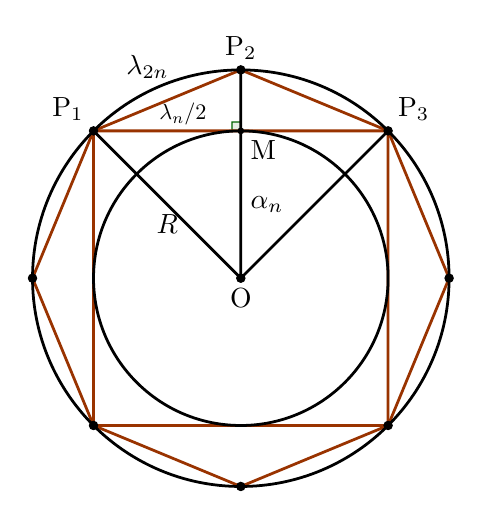
\begin{tikzpicture}[scale=.75]
\tkzSetUpLine[line width=1pt,color=black]
\tkzSetUpPoint[fill=black]

\tkzDefPoints{0/0/P0}
\tkzDefPoint(22.5:2.7){P1}

\tkzDefRegPolygon[side,sides=8](P0,P1)

\tkzDefCircle[circum](P1,P2,P3) \tkzGetPoint{O}
\tkzInterLL(O,P5)(P4,P6) \tkzGetPoint{M}

\tkzFillPolygon[fill=white](P1,P2,P3,P4,P5,P6,P7,P8)

\tkzMarkRightAngles[line width=0.5pt, size=.15,color=AngleClr,fill=AngleClr,fill opacity=0.1](P5,M,P6)

\tkzDrawPolygon[color=ShapeClr](P1,P2,P3,P4,P5,P6,P7,P8)
\tkzDrawPolygon[color=ShapeClr](P2,P4,P6,P8)


\tkzDrawCircle[line width=1pt,black](O,P1)
\tkzDrawCircle[line width=1pt,black](O,M)
\tkzDrawSegments(O,P6 O,P4 O,P5)

\tkzLabelSegment(O,P6){$R$}
\tkzLabelSegment[yshift=0.45cm,xshift=0.2cm,scale=0.8](P6,M){$\lambda_n/2$}
\tkzLabelSegment[yshift=0.7cm,xshift=-0.25cm](P6,P5){$\lambda_{2n}$}
\tkzLabelSegment[right](O,M){$\alpha_n$}

\tkzDrawPoints[size=3](P1,P2,P3,P4,P5,P6,P7,P8,O)
\tkzDrawPoints[size=2](M)

\tkzLabelPoint[below](O){$\rm O$}
\tkzLabelPoint[below right](M){$\rm M$}
\tkzLabelPoint[above left](P6){$\rm P_1$}
\tkzLabelPoint[above](P5){$\rm P_2$}
\tkzLabelPoint[above right](P4){$\rm P_3$}

\end{tikzpicture}

\end{document}
